% !TeX spellcheck = en_US
% !TeX encoding = utf8
% !TeX program = xelatex
% !BIB program = bibtex
% \documentclass[mathserif,compress,12pt]{ctexbeamer}
\documentclass[12pt,notes,mathserif]{beamer}
% \documentclass[draft]{beamer}	
\usetheme{Singapore}
% \usetheme{Hannover}
%\usepackage{pgfpages}
%\setbeameroption{show notes on second screen}

\usepackage[british]{babel}
\usepackage{graphicx,hyperref,url}
% \usepackage{ru}
\usepackage{mmstyles,bm,ulem}

\usepackage{listings}
\usefonttheme[onlymath]{serif}
\usepackage{fontspec}
\usepackage{xeCJK}
% \setCJKfamilyfont{hei}{SimHei}
% \setCJKmainfont[BoldFont=Arial, ItalicFont=Arial]{Arial}
% \pgfdeclareimage[width=\paperwidth,height=\paperheight]{bg}{background}
% \setbeamertemplate{background}{\pgfuseimage{bg}}
%% columns
\newcommand{\begincols}[1]{\begin{columns}{#1}}
\newcommand{\stopcols}{\end{columns}}
% \usepackage[backend=biber]{biblatex}
% \bibliography{./ref.bib}
%\addbibresource{ref.bib}
\usepackage{indentfirst}
\usepackage{longtable}
\usepackage{float}
%\usepackage{picins}
\usepackage{rotating}
\usepackage{subfigure}
\usepackage{tabu}
\usepackage{amsmath}
\usepackage{amssymb}
\usepackage{setspace}
\usepackage{amsfonts}
\usepackage{appendix}
\usepackage{listings}
\usepackage{xcolor}
\usepackage{colortbl}
\usepackage{geometry}
% \setCJKfamilyfont{cjkhwxk}{SimSun}
% \newcommand*{\cjkhwxk}{\CJKfamily{cjkhwxk}}
%\newfontfamily{\consolas}{Consolas}
%\newfontfamily{\monaco}{Monaco}
%\setmonofont[Mapping={}]{Consolas}	%英文引号之类的正常显示,相当于设置英文字体
%\setsansfont{Consolas} %设置英文字体 Monaco, Consolas,  Fantasque Sans Mono
% \setmainfont{Times New Roman}
% \newfontfamily{\consolas}{Times New Roman}
% \newfontfamily{\monaco}{Arial}
% \setCJKmainfont{Times New Roman}
%\setmainfont{MONACO.TTF}
%\setsansfont{MONACO.TTF}
\newcommand{\verylarge}{\fontsize{60pt}{\baselineskip}\selectfont}  
\newcommand{\chuhao}{\fontsize{44.9pt}{\baselineskip}\selectfont}  
\newcommand{\xiaochu}{\fontsize{38.5pt}{\baselineskip}\selectfont}  
\newcommand{\yihao}{\fontsize{27.8pt}{\baselineskip}\selectfont}  
\newcommand{\xiaoyi}{\fontsize{25.7pt}{\baselineskip}\selectfont}  
\newcommand{\erhao}{\fontsize{23.5pt}{\baselineskip}\selectfont}  
\newcommand{\xiaoerhao}{\fontsize{19.3pt}{\baselineskip}\selectfont} 
\newcommand{\sihao}{\fontsize{14pt}{\baselineskip}\selectfont}      % 字号设置  
\newcommand{\xiaosihao}{\fontsize{12pt}{\baselineskip}\selectfont}  % 字号设置  
\newcommand{\wuhao}{\fontsize{10.5pt}{\baselineskip}\selectfont}    % 字号设置  
\newcommand{\xiaowuhao}{\fontsize{9pt}{\baselineskip}\selectfont}   % 字号设置  
\newcommand{\liuhao}{\fontsize{7.875pt}{\baselineskip}\selectfont}  % 字号设置  
\newcommand{\qihao}{\fontsize{5.25pt}{\baselineskip}\selectfont}    % 字号设置 

\graphicspath{{./fig/}}

% \setbeamertemplate{footnote}{%
%   \hangpara{2em}{1}%
%   \makebox[2em][l]{\insertfootnotemark}\footnotesize\insertfootnotetext\par%
% }

\definecolor{cred}{rgb}{0.6,0,0}
\definecolor{cgreen}{rgb}{0.25,0.5,0.35}
\definecolor{cpurple}{rgb}{0.5,0,0.35}
\definecolor{cdocblue}{rgb}{0.25,0.35,0.75}
\definecolor{cdark}{rgb}{0.95,1.0,1.0}
\lstset{
	language=R,
	numbers=left,
	numberstyle=\tiny\color{black},
	keywordstyle=\color{cpurple}\consolas,
	commentstyle=\color{cgreen}\consolas,
	stringstyle=\color{cred}\consolas,
	frame=single,
	escapeinside=``,
	xleftmargin=1em,
	xrightmargin=1em, 
	backgroundcolor=\color{cdark},
	aboveskip=1em,
	breaklines=true,
	tabsize=3
} 

\providecommand{\tightlist}{%
  \setlength{\itemsep}{0pt}\setlength{\parskip}{0pt}}

  
% The title of the presentation:
%  - first a short version which is visible at the bottom of each slide;
%  - second the full title shown on the title slide;
% \title[]{\LARGE CSE 5526: Introduction to Neural Networks}

% Optional: a subtitle to be dispalyed on the title slide
\title{ Support Vector Machines (SVMs)\\Part 4: Non-separable data}

% The author(s) of the presentation:
%  - again first a short version to be displayed at the bottom;
%  - next the full list of authors, which may include contact information;
 
\author[YingmingLi]{Yingming Li \\ yingming@zju.edu.cn}
% The institute:
%  - to start the name of the university as displayed on the top of each slide
%    this can be adjusted such that you can also create a Dutch version
%  - next the institute information as displayed on the title slide

\institute[DSERC, ZJU]{Data Science \& Engineering Research Center, ZJU}
% Add a date and possibly the name of the event to the slides
%  - again first a short version to be shown at the bottom of each slide
%  - second the full date and event name for the title slide
\begin{document}

\AtBeginSection[]
{
	\begin{frame}
		\frametitle{Outline}
		\tableofcontents[currentsection]
	\end{frame}
}

% \AtBeginSubsection[2-]
% {
%    \begin{frame}
%        \frametitle{Outline}
%        \tableofcontents[currentsection]
%    \end{frame}
% }
\begin{frame}[c]
	\titlepage
	% \begin{center}
		% MLP Tips
	% \end{center}
\end{frame}

% 2
\begin{frame}[c]
\frametitle{What if the classes overlap?}
\begin{itemize}
\item  Allow mis-classifications, but penalize them
\begin{itemize}
\item  in proportion to distance on the wrong side of the margin
\item  Add to existing cost, minimize sum of the two
\end{itemize}
\item Introduce ``slack variables'' $\xi_p\geqslant{}0$
\begin{itemize}
\item one per training point
\item $\xi_p=\max (1-d_py(\mathbf{x}_p),0)$
\end{itemize}
\item Interpretation
\begin{itemize}
\item $\xi_p=0$ for points on the correct side of the margin
\item $0<\xi_p < 1$ for correctly classified points within margin
\item $\xi_p>1$ for mis-classified points
\end{itemize}
\end{itemize}
\end{frame}


% 3
\begin{frame}[c]
\frametitle{Meaning of $\xi_p$}
\begin{center}
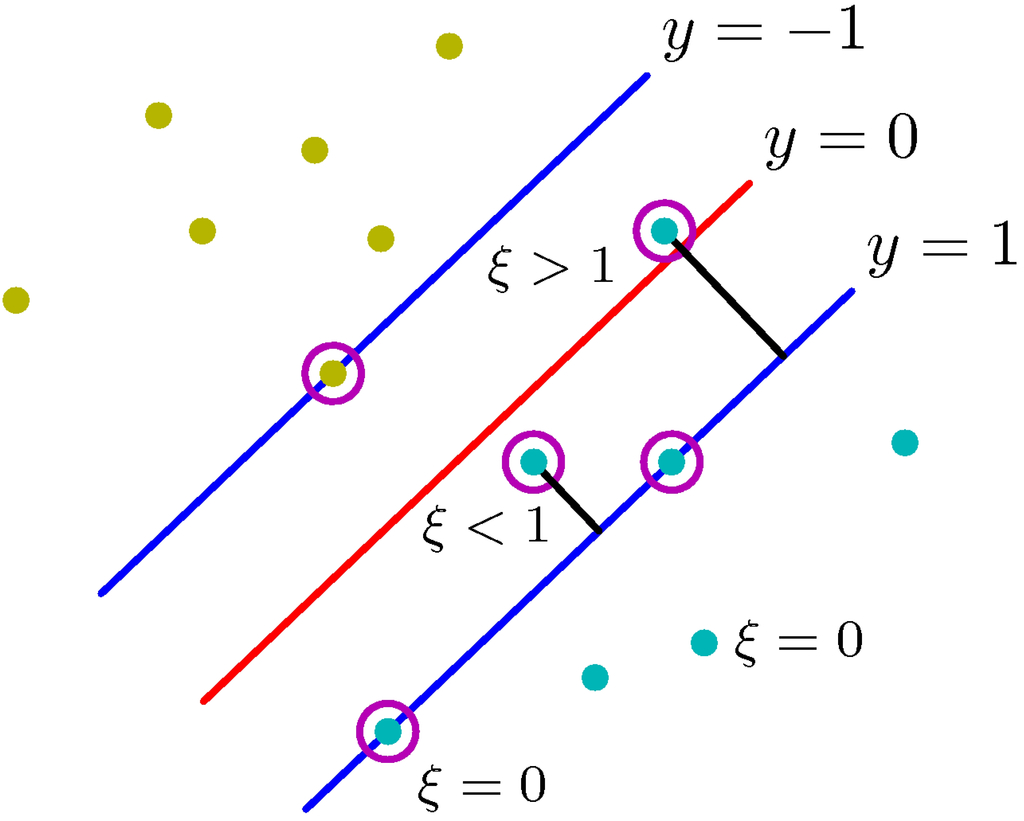
\includegraphics[width=0.7\linewidth]{fig10/lec113.jpg}
\end{center}
\end{frame}

% 4
\begin{frame}[c]
\frametitle{Incorporate slack variables in optimization}
\begin{itemize}
\item New problem:


$$\argmin_{\mathbf{w},b}  \frac{1}{2} ||\mathbf{w}||^2+C\sum_p\xi_p$$
$$\text{\textit{s.t.} }  d_py(\mathbf{x}_p)\geqslant{}1-\xi_p$$

\item So constraint $d_py(\mathbf{x}_p)\geqslant{}1$ has been relaxed
\item But now minimize the sum of the 𝜉$\xi_p$ too
\item $C$ controls trade-off between margin and slack
\begin{itemize}
\item As $C\to \infty$, return to SVM for separable data
\end{itemize}
\end{itemize}
\end{frame}

% 5
\begin{frame}[c]
\frametitle{New primal Lagrangian adds two new terms}
\begin{itemize}
\item Primal Lagrangian (still QP with linear constraints):
\begin{eqnarray*}
L(\mathbf{w},b,\mathbf{a},\mathbf{\mu}) &=\dfrac{1}{2}||\mathbf{w}||^2+C\sum_p\xi_p-\sum_p\mu_p\xi_p\\
\quad & +\sum_pa_p(d_p(\mathbf{w}^t\mathbf{x}_p+b)-1+\xi_p)
\end{eqnarray*}
\item KKT conditions:
\[\begin{matrix}
a_p\geqslant{}0 &\xi_p\geqslant{}0\\
d_py(\mathbf{x}_p)-1+\xi_p\geqslant{}0&\mu_p\geqslant{}0\\
a_p(d_py(\mathbf{x}_p)-1+\xi_p)=0&\mu_p\xi_p=0
\end{matrix}\]
\end{itemize}
\end{frame}

% 6
\begin{frame}[c]
\frametitle{Derive dual Lagrangian by solving for $\mathbf{w}$, $b$, $\mathbf{\xi}$}
\begin{itemize}
\item The matrix
\[
\begin{matrix}
\dfrac{\partial L}{\partial \mathbf{w}}=0 \Rightarrow \mathbf{w}=\sum\limits_pa_pd_p\mathbf{x}_p&\text{Unchanged}\\
\dfrac{\partial L}{\partial b}=0 \Rightarrow \mathbf{w}=\sum\limits_pa_pd_p=0&\text{Unchanged}\\
\dfrac{\partial L}{\partial \xi_p}=0 \Rightarrow a_p=C-\mu_p&\text{New}\\
\end{matrix}
\]
\item So $\mathbf{\mu}$ can be replaceed by $\mathbf{a}$
\end{itemize}
\end{frame}



% 7
\begin{frame}[c]
\frametitle{New dual Lagrangian changed very little}
\begin{itemize}
\item Dual Lagrangian
\begin{gather*}
\tilde{L}(\mathbf{a})=\sum_pa_p-\dfrac{1}{2}\sum_p\sum_qa_pa_qd_pd_q\mathbf{x}_p^T\mathbf{x}_q
\end{gather*}
\item With constraints
\[\begin{matrix}
0\leqslant{}a_p\leqslant{}C&\sum\limits_pa_pd_p=0
\end{matrix}\]
\item Only difference is upper bound on $a_p$ from $\mu_p \geqslant{}0$
\item Still a quadratic program with linear constraints
\item Predictions still made identically
\end{itemize}
\end{frame}



% 8
\begin{frame}[c]
\frametitle{Now many types of points}
\begin{itemize}
\item Points with $a_p= 0$ are still non-support vectors
\begin{itemize}
\item Do not contribute to classification
\end{itemize}
\item Points with $a_p>0$
\begin{itemize}
\item Must satisfy KKT condition $d_py(x_p)=1-\xi_p$
\item Points with $0 < a_p < C$ have margin 1
\begin{itemize}
\item KKT condition that $\xi_p=0$
\end{itemize}
\item Points with $a_p=C$ can lie inside the margin
\begin{itemize}
\item Correctly classfied if $\xi_p\leqslant{}1$
\item Incorrectly classified if $\xi_p>1$
\end{itemize}
\end{itemize}
\end{itemize}
\end{frame}


% 9
\begin{frame}[c]
\frametitle{Remarks on points with $a_p=C$}
\begin{itemize}
\item It is undesirable that these points are support vectors
\item All misclassified training points must be SVs
\item Makes decisions sensitive to outliers in training
\item Need to evaluate kernel on them at test time
\end{itemize}
\end{frame}



% 10
\begin{frame}[c]
\frametitle{SVM double-moon training set, $d=-6$}
\begin{center}
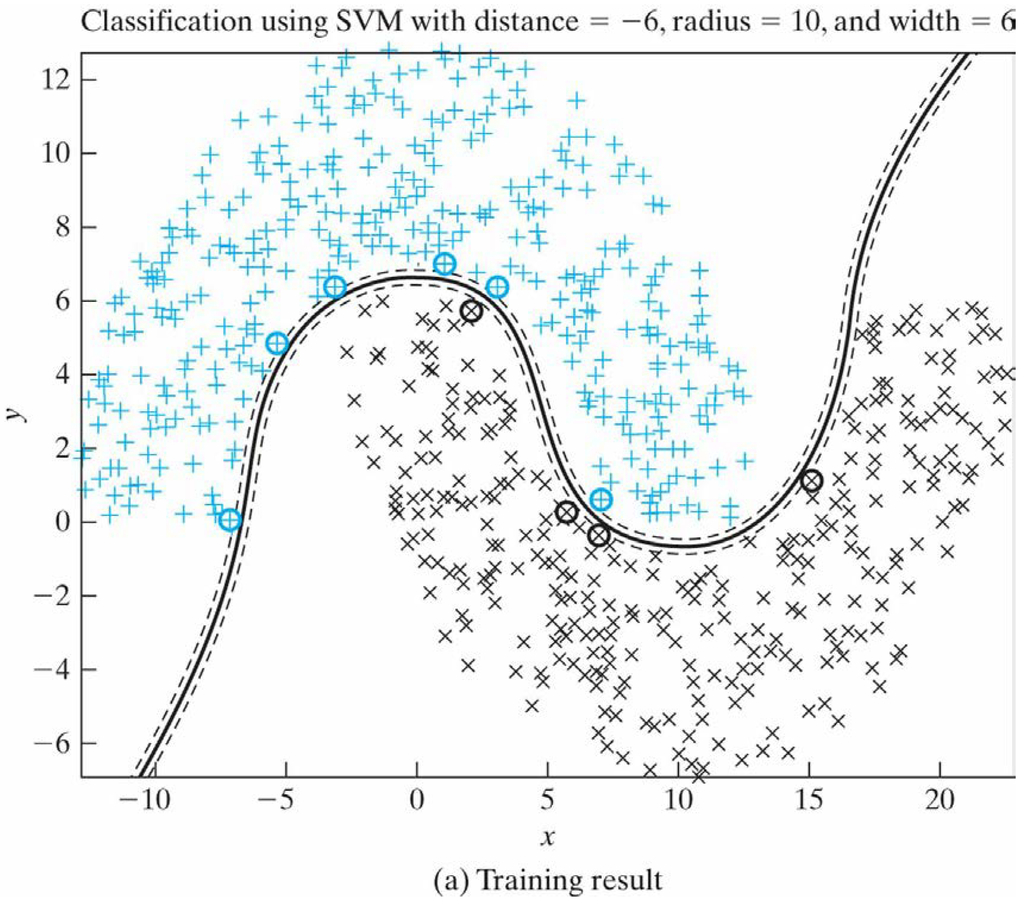
\includegraphics[width=0.7\linewidth]{fig10/lec1110.jpg}
\end{center}
\end{frame}


% 11
\begin{frame}[c]
\frametitle{SVM double-moon test set, $d=-6$}
\begin{center}
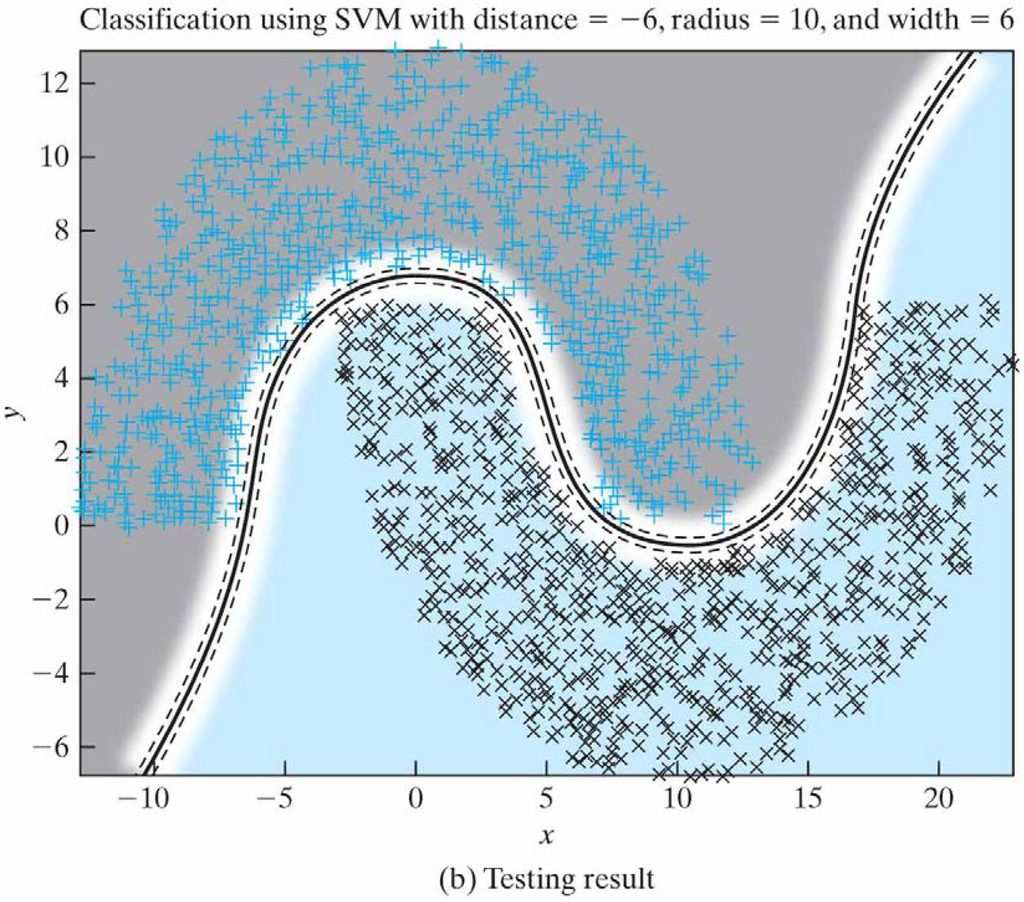
\includegraphics[width=0.7\linewidth]{fig10/lec1111.jpg}
\end{center}
\end{frame}



\begin{frame}
\begin{center}
\chuhao Thank you! %\fontspec{LHANDW.TTF}
\end{center}
\end{frame}
\end{document}
